\documentclass{article}
%\usepackage{geometry}
%\geometry{top = 1in, bottom = 1in, left = 1in, right = 1in}
\usepackage[top = 0.7in, bottom = 0.7in, left = 0.7in, right = 0.7in]{geometry}
\usepackage{amsmath,amssymb,amsthm,mathrsfs}
\usepackage{graphicx}
\usepackage{bm}
\usepackage{float}
\usepackage[font=footnotesize,labelfont=bf]{caption}
\usepackage{movie15}
\usepackage{hyperref}

\usepackage{fancyhdr}
\pagestyle{fancy}
\rhead{\footnotesize {08/30/2012 ; MESA version 4411} }
\chead{\footnotesize {Authors: Jared Brooks, Lars Bildsten, Bill Paxton} }
\lhead{\footnotesize {mesa/star/test\_suite/create\_zahb} }

\begin{document}
	
	\begin{center}
	  \begin{Large}
	    \textbf{CREATE ZAHB}\\
	  \end{Large}
	\end{center}

        This test is to show the evolution of a few different mass pre-ZAHB stars into ZAHB stars.  A list of masses (\texttt{masses\_filename = 'zahb\_masses.list'}) is read in, and for each mass, \texttt{MESA} takes a pre-saved model named \texttt{pre\_zahb.mod} and relaxes its mass and evolves it until the mass fraction for center helium drops below the \texttt{HB\_limit}, which, is set in \texttt{inlist\_create\_zahb} to 0.9.\\

        In addition to the \texttt{HB\_limit}, the inlist contains a few other important controls.  These include some mixing controls (\texttt{mixing\_length\_alpha = 1.9 ; use\_Henyey\_MLT = .true.}), atmosphere option (\texttt{which\_atm\_option = 'photosph\-ere\_tables'}), and some opacity controls.\\

        The file (\texttt{zahb\_masses.list}) contains three masses: $0.49 M_\odot$, $0.70 M_\odot$, and $1.2 M_\odot$.  Each one is run consecutively in the order listed, and all the log files from each run are stored in the same \texttt{LOGS/} directory.  To differentiate the log files from each run, they are named with prefixes, such as \texttt{i001\_history.data} and \texttt{i001\_log1.data} for the first run, \texttt{i002\_history.data} and \texttt{i002\_log1.data} for the second run, etc.\\

        Since all these models derive from the same \texttt{pre\_zahb.mod}, they all have very similar cores.  The plot below, which shows the evolution of the center temperature and density (figure \ref{fig:1}), is nearly identical for each run.


        \begin{figure}[H]
          \centering
          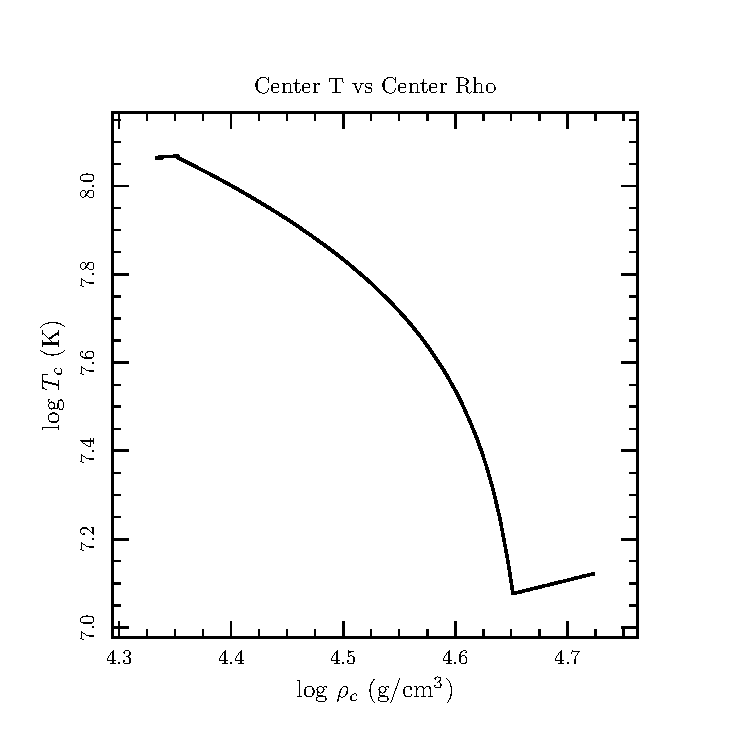
\includegraphics[width = 5in]{/Users/jaredbrooks/create_zahb/plots_out/Tc_vs_Rhoc_1.pdf}
          \caption{Evolution of center temperature and density, same for all runs}
          \label{fig:1}
        \end{figure}

        \pagebreak

        The important difference between these models is the size of the envelope.  Below are abundance and burning rate profiles from the end of each run.  First is the $0.49 M_\odot$ model (figures \ref{fig:2} and \ref{fig:3}).

        \begin{figure}[H]
          \begin{minipage}[b]{0.5\linewidth}
	    \centering
	    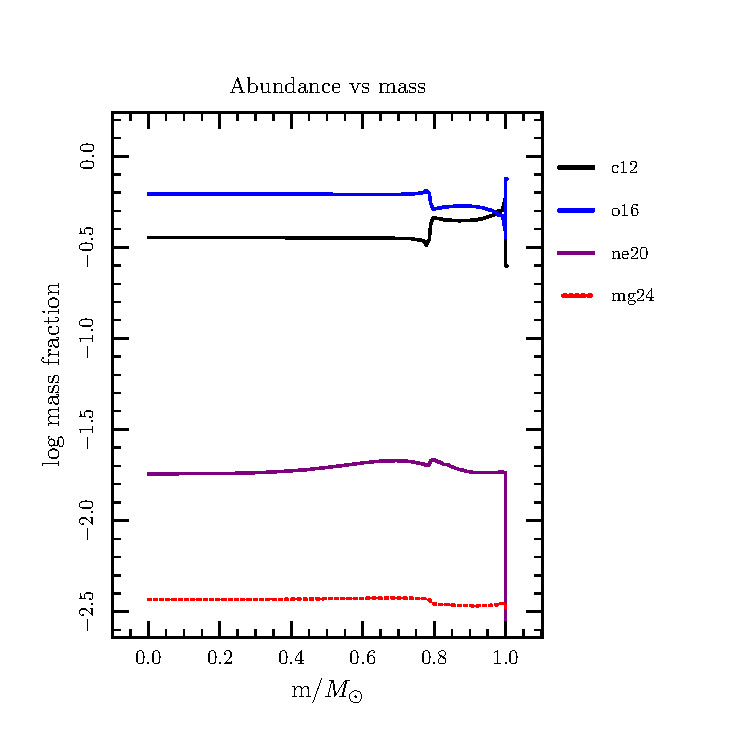
\includegraphics[width = 3.8in]{/Users/jaredbrooks/create_zahb/plots_out/Abundance_vs_mass_1.pdf}
	    \caption{$0.49 M_\odot$ Abundance profile from end of run}
	    \label{fig:2}
          \end{minipage}
          \hspace{0cm}
          \begin{minipage}[b]{0.5\linewidth}
            \centering
            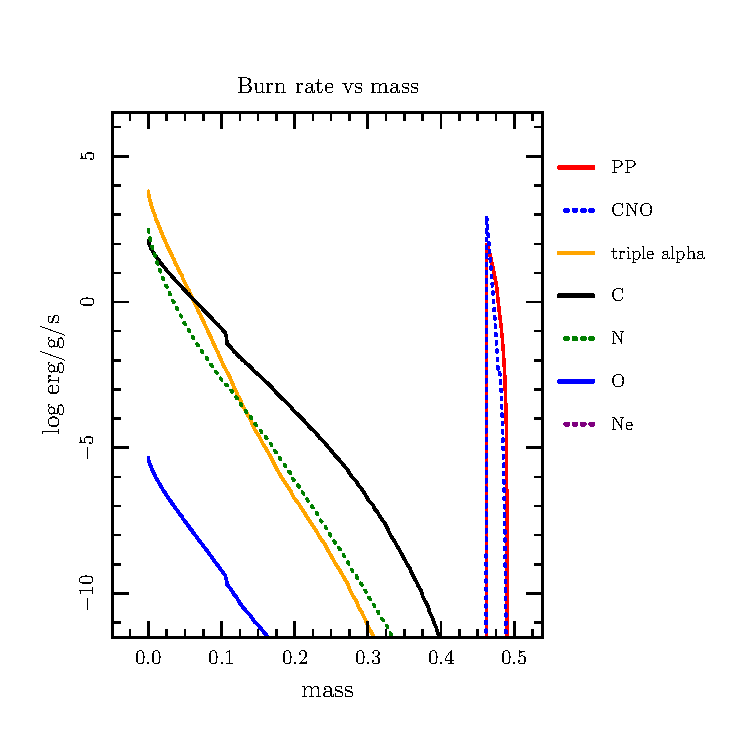
\includegraphics[width = 3.8in]{/Users/jaredbrooks/create_zahb/plots_out/Burnrate_vs_mass_1.pdf}
            \caption{$0.49 M_\odot$ burning rate profile from end of run}
            \label{fig:3}
          \end{minipage}
	\end{figure}

        Next is the $0.70 M_\odot$ model (figures \ref{fig:4}and \ref{fig:5}).

        \begin{figure}[H]
          \begin{minipage}[b]{0.5\linewidth}
            \centering
            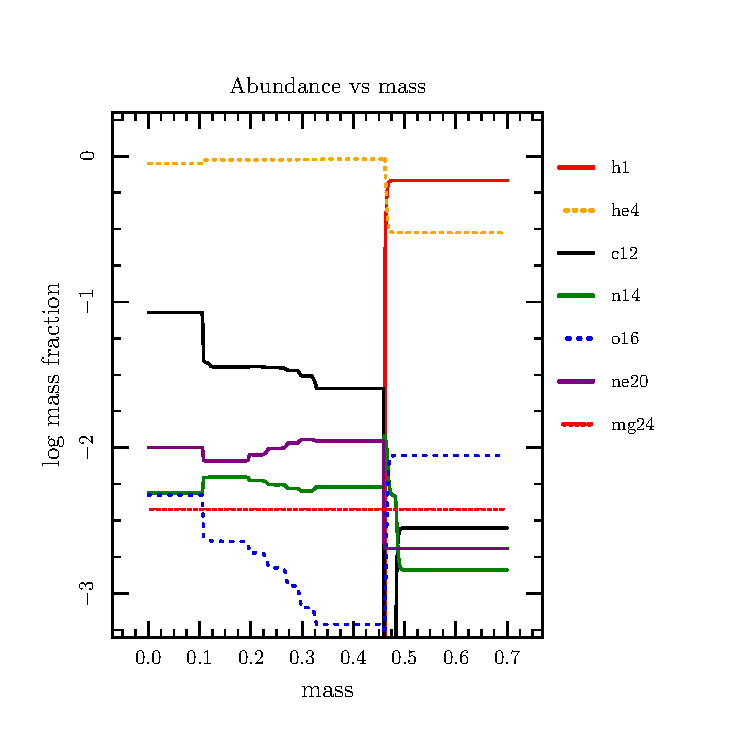
\includegraphics[width = 3.8in]{/Users/jaredbrooks/create_zahb/plots_out/Abundance_vs_mass_2.pdf}
            \caption{$0.70 M_\odot$ Abundance profile from end of run}
            \label{fig:4}
          \end{minipage}
          \hspace{0cm}
          \begin{minipage}[b]{0.5\linewidth}
            \centering
            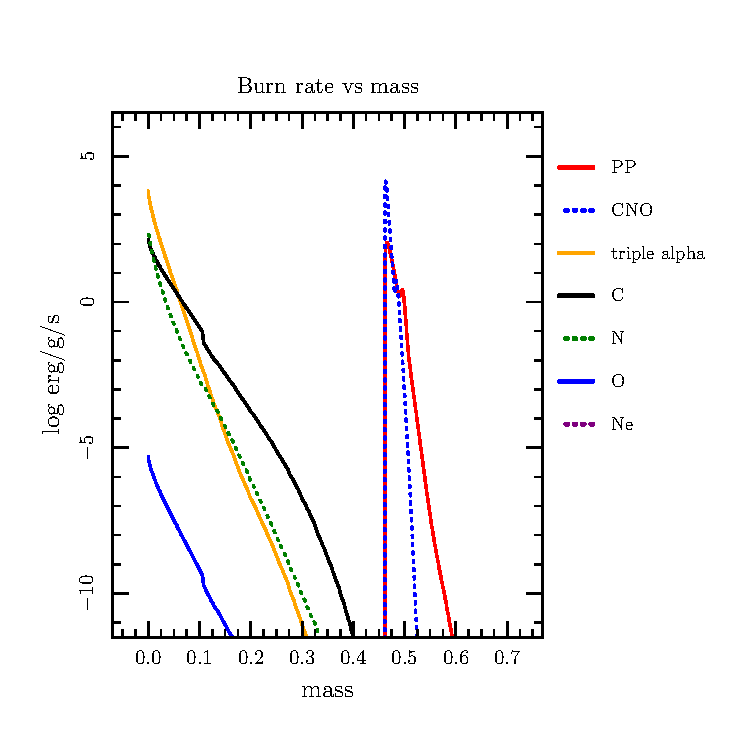
\includegraphics[width = 3.8in]{/Users/jaredbrooks/create_zahb/plots_out/Burnrate_vs_mass_2.pdf}
            \caption{$0.70 M_\odot$ burning rate profile from end of run}
            \label{fig:5}
          \end{minipage}
        \end{figure}

        \pagebreak

        Finally, the $1.2 M_\odot$ model (figures \ref{fig:6}and \ref{fig:7}).

        \begin{figure}[H]
          \begin{minipage}[b]{0.5\linewidth}
            \centering
            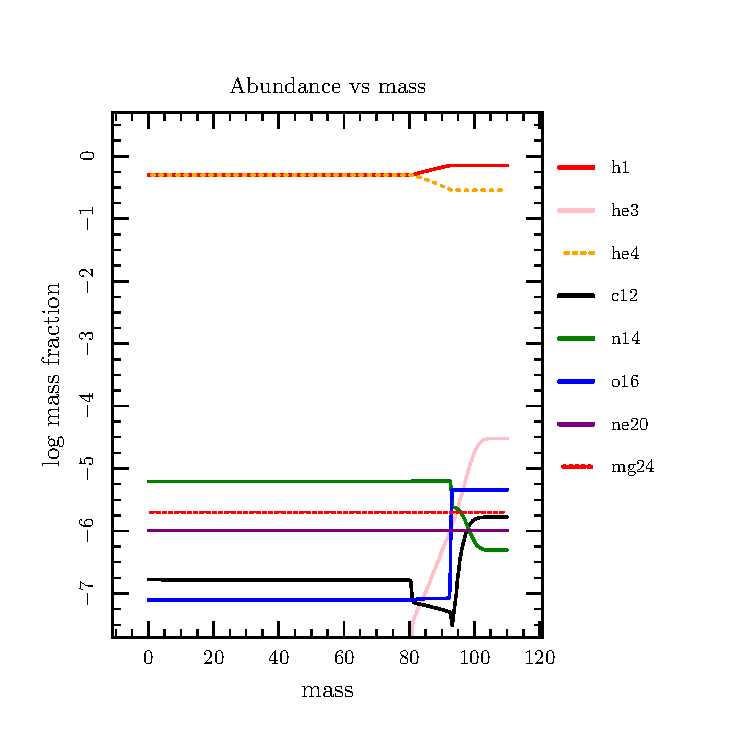
\includegraphics[width = 3.8in]{/Users/jaredbrooks/create_zahb/plots_out/Abundance_vs_mass_3.pdf}
            \caption{$1.2 M_\odot$ Abundance profile from end of run}
            \label{fig:6}
          \end{minipage}
          \hspace{0cm}
          \begin{minipage}[b]{0.5\linewidth}
            \centering
            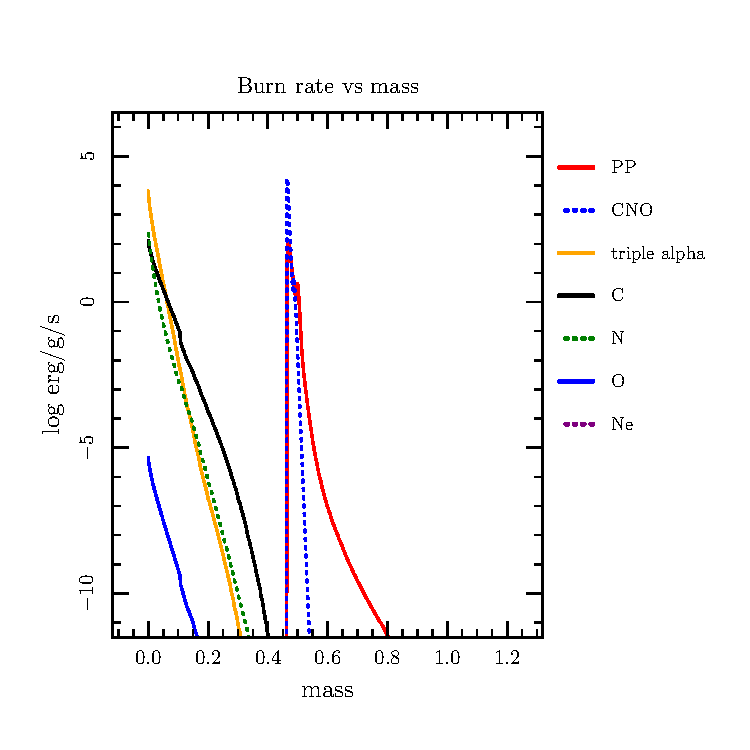
\includegraphics[width = 3.8in]{/Users/jaredbrooks/create_zahb/plots_out/Burnrate_vs_mass_3.pdf}
            \caption{$1.2 M_\odot$ burning rate profile from end of run}
            \label{fig:7}
          \end{minipage}
        \end{figure}

        \pagebreak

        Since all the models have very similar cores, and the ending condition (\texttt{HB\_limit}) depends on the core, the models have similar evolution times, about 5 Myr.  Therefore, we can construct an isochrone on the HR-diagram.  The isochrone below (figure \ref{fig:8}) was constructed from running the test case with \texttt{zahb\_masses.list\_big}, instead of \texttt{zahb\_masses.list}, which has 18 masses, but with the same range ($0.49 M_\odot$ to $1.2 M_\odot$), and plotting the ending luminosity and effective temperature from each model.

        \begin{figure}[H]
          \centering
          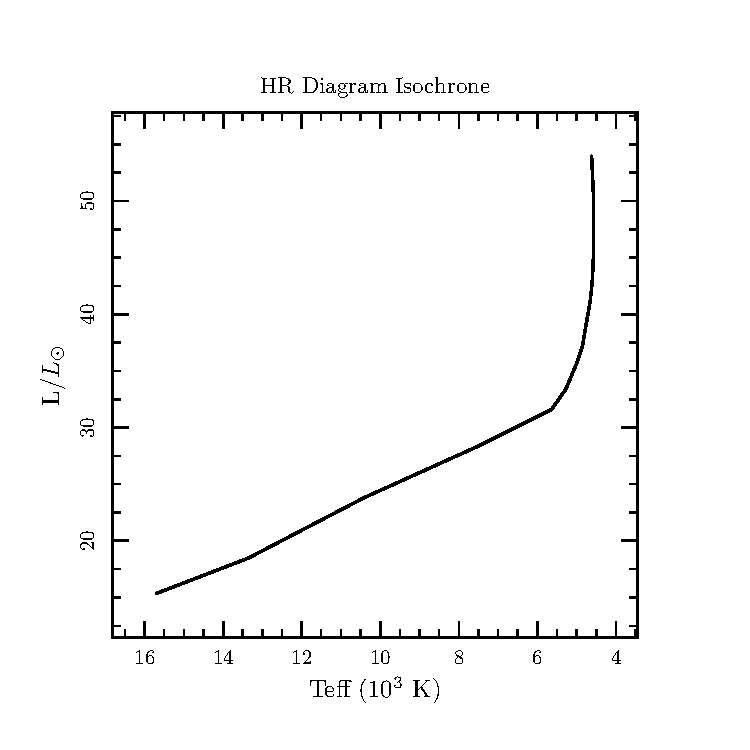
\includegraphics[width = 5in]{/Users/jaredbrooks/create_zahb/plots_out/Isochrone_1.pdf}
          \caption{Isochrone of ZAHB stars from $0.49 M_\odot$ to $1.2 M_\odot$}
          \label{fig:8}
        \end{figure}


\end{document}
